
\medskip

%\begin{center}
%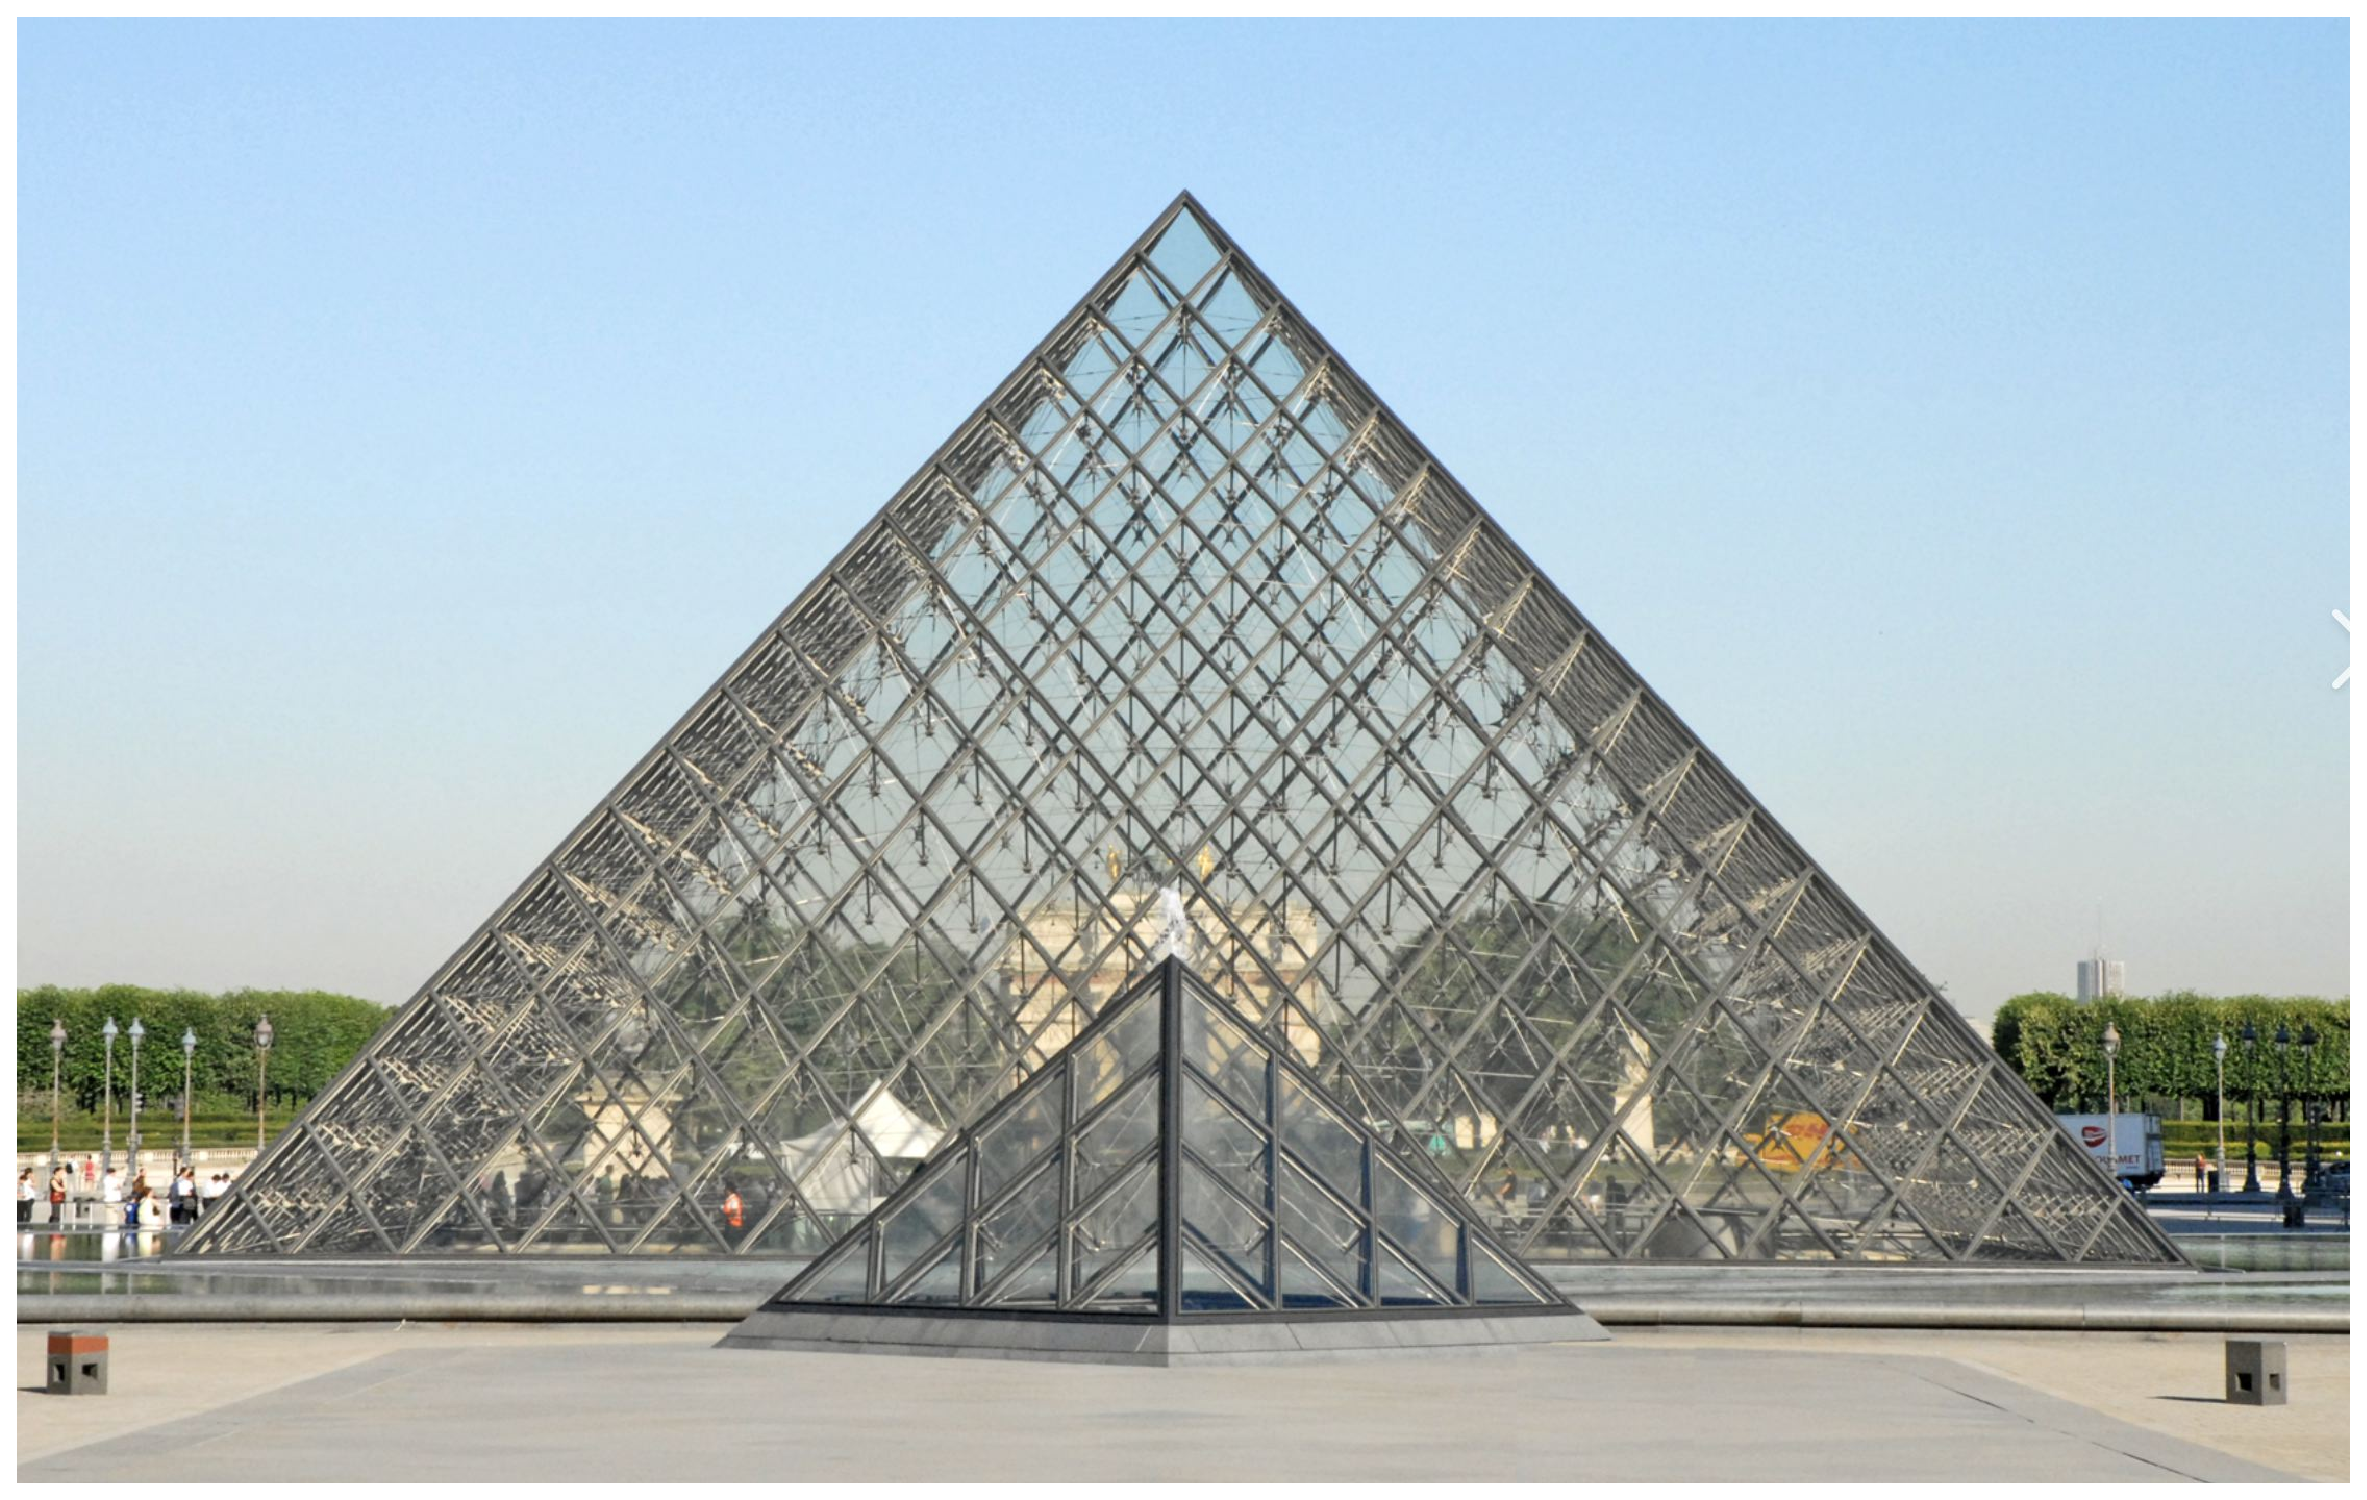
\includegraphics[width=6cm]{pyramide_Polynesie_2019}
%\end{center}
%
%La pyramide du Louvre à Paris est une pyramide à base carrée de côté 35,4~m et de hauteur
%21,6~m.
%
%C'est une réduction de la pyramide de Khéops en Egypte, qui mesure environ 230,5~m de côté.
%
%\medskip

\begin{enumerate}
\item %Montrer que la hauteur de la pyramide de Khéops est d'environ 140,6~m.

Si $k$ est la hauteur de la pyramide de Khéops, on a : $\dfrac{35,4}{230,5} = \dfrac{21,6}{k}$, soit $35,4k = 230,5 \times 21,6$ et enfin $k = \dfrac{230,5 \times 21,6}{35,4} \approx 140,644$, soit environ 140,6~m au dixième près.
\item %Calculer le volume en m$^3$ de la pyramide du Louvre. (Arrondir à l'unité)
Le volume de la pyramide du Louvre est égal à $35,4 \times 35,4 \times 21,6  \times \dfrac{1}{3} = \np{1253,16} \times 7,2 = \np{9022,75}$~m$^3$, soit \np{9023}~m$^3$ à l'unité près.
\item %Par quel nombre peut-on multiplier le volume de la pyramide du Louvre pour obtenir celui de la pyramide de Khéops ? (Arrondir à l'unité)
La pyramide de Khéops est $\dfrac{230,5}{35,4}$ fois plus grande que la pyramide du Lovre, donc son volume est $\left(\dfrac{230,5}{35,4}\right)^3 = 276,06$ plus grand.

La pyramide de Khéops peut donc contenir à peu près 276 pyramides du Louvre.
\end{enumerate}

\medskip

\textbf{Rappel:}

Volume d'une pyramide $ =  \dfrac{\text{Aire de la base} \times \text{Hauteur}}{3}$.

\bigskip

